%
% cwt.tex
%
% (c) 2019 Prof Dr Adreas Müller, Hochschule Rapperswil
%

%
% Definition der stetigen Wavelet-Transformation
%
\begin{frame}
\frametitle{Stetige Wavelet Transformation (CWT)}
Analyse mit verschobenen und gestreckten Kopien von $\psi$:
\[
\psi_{a,b}(t)
=
T_bD_a\psi(t)
=
\frac{1}{\sqrt{|a|}}\psi\biggl(\frac{t-b}{a}\biggr)
\]
\vspace{-10pt}
\begin{itemize}
\item<2-> Translation um $b$
\item<3-> Dilatation mit $a\ne 0$\uncover<4->{, $a<0$ $\Rightarrow$ mit Spiegelung}
\end{itemize}
\uncover<5->{%
\begin{definition}[Stetige Wavelet Transformation]
Für ein Wavelet $\psi$ ist 
die Stetige Wavelet-Transformation eines Signals $f(t)$ die Funktion 
von zwei Variablen $(a,b)\in\mathbb R^*\times\mathbb R$
\begin{align*}
\mathcal{W}f(a,b)
=
\mathcal{W}_{\psi}f(a,b)
&=
\langle f,\psi_{a,b}\rangle
=
\langle f, T_bD_a\psi\rangle
\\
&\uncover<6->{=
\frac{1}{\sqrt{|a|}}
\int_{-\infty}^{\infty} f(t) \overline{\psi\biggl(\frac{t-b}{a}\biggr)}\,dt.}
\end{align*}
\end{definition}
}%
\end{frame}

\definecolor{mexican}{rgb}{0.6,0,0.6}
\def\s{0.4}
\def\mexikanerhut#1#2{
	\draw[color=mexican,line width=1pt] plot[domain=-5:5,samples=100]
		({((#1)*\x+(#2))},{\s*(1-\x*\x)*exp(-\x*\x/2)/sqrt(#1)+(#1/0.6)*0.75*11});
	\fill[color=mexican] ({#2},{(#1/0.6)*0.75*11}) circle[radius=0.1];
}

%
% Beispiel: Analyse mit Mexicanerhut
%
\begin{frame}
\frametitle{Beispiel: Analyse mit Mexikanerhut}
\centering
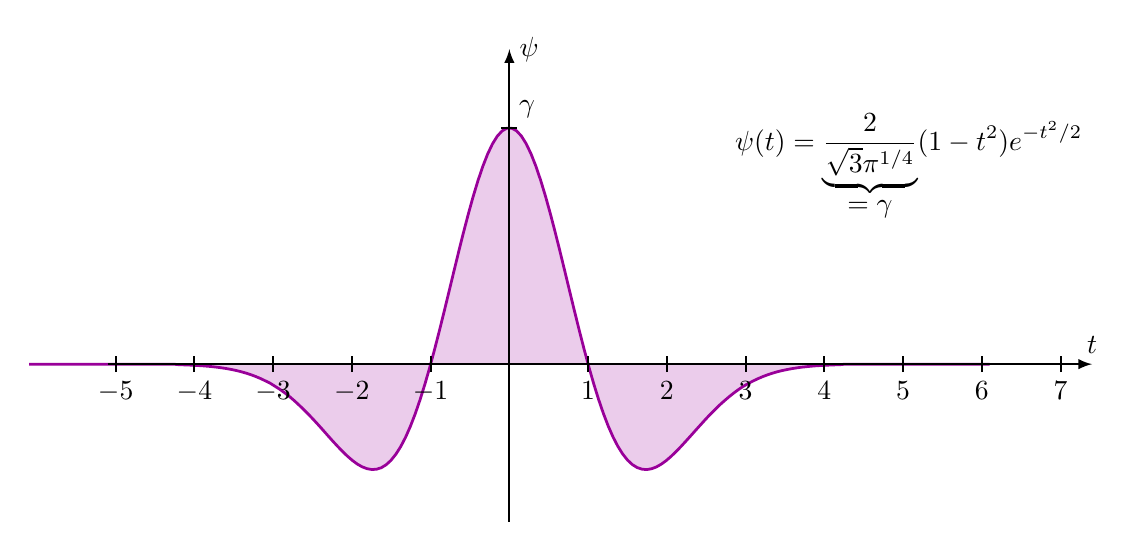
\begin{tikzpicture}[>=latex]

\fill[color=mexican!20] plot[domain=-6.1:6.1,samples=200]
        ({\x},{3*(1-\x*\x)*exp(-\x*\x/2)})--cycle;
\draw[line width=1pt,color=mexican] plot[domain=-6.1:6.1,samples=200]
        ({\x},{3*(1-\x*\x)*exp(-\x*\x/2)});

\draw[->,line width=0.7pt] (-5.1,0)--(7.4,0) coordinate[label=$t$];
\draw[->,line width=0.7pt] (0,-2)--(0,4) coordinate[label={right:$\psi$}];

\foreach \x in{1,...,7}{
        \draw[line width=0.7pt] ({\x},-0.1)--({\x},0.1);
        \node at ({\x},-0.1) [below] {$\x$};
}
\foreach \x in{1,...,5}{
        \draw[line width=0.7pt] ({-\x},-0.1)--({-\x},0.1);
        \node at ({-\x},-0.1) [below] {$-\x$};
}
\node at (7.4,2.5) [left] {$\psi(t) = \displaystyle\underbrace{\frac{2}{\sqrt{3}\pi^{1/4}}}_{\displaystyle=\gamma} (1-t^2)e^{-t^2/2}$};
\node at (0,3) [above right] {$\gamma$};
\draw[line width=1pt] (-0.1,3)--(0.1,3);
\end{tikzpicture}
\end{frame}

\ifthenelse{\boolean{presentation}}{

\newboolean{examples}
\setboolean{examples}{true}
\ifthenelse{\boolean{examples}}{

%
% Beispiel
%
\begin{frame}
\begin{center}
\begin{tikzpicture}[>=latex,scale=0.8181]

\uncover<3,5,7,9,11,13,15,17,19,21,23,25,26>{%
\node at (1.5,{0.375*11}) {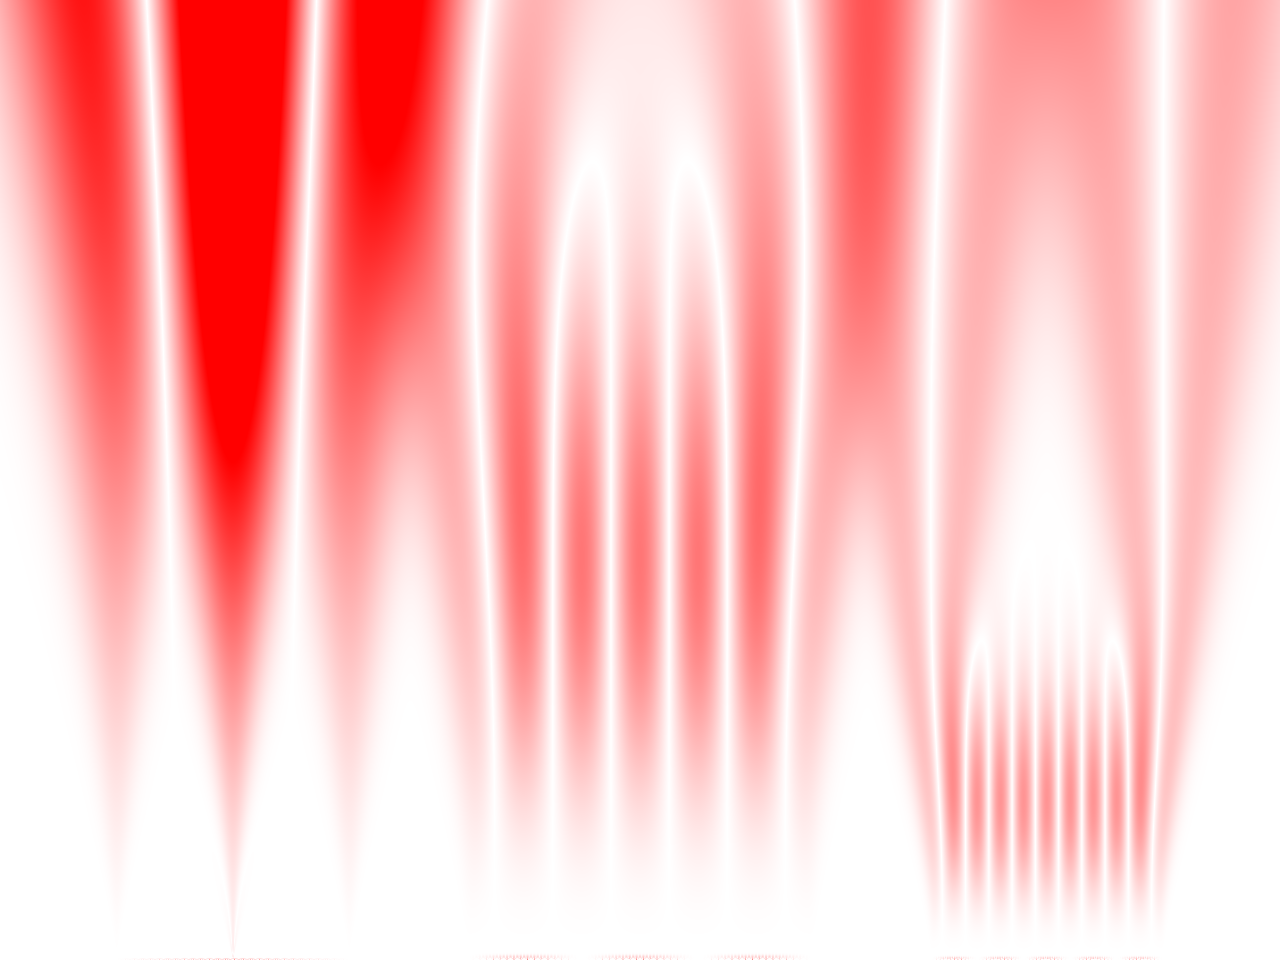
\includegraphics[width=9cm]{../../buch/chapters/4-cwt/images/notes.png}};
}

\only<1,2,4,6,8,10,12,14,16,18,20,22,24>{
\draw[->,line width=0.7pt] (-4.1,0)--(7.3,0) coordinate[label={$t$}];
\draw[->,line width=0.7pt] (0,-0.1)--(0,{0.75*11+0.3})
        coordinate[label={right:$f(t)\mathstrut$}];
}

\draw[line width=1pt,color=blue]
	(-4.1,0)--(-3,0)--(-2,{2*2.883})--(-1,0)--(0,0)--
        plot[domain=0:3,samples=100] ({\x},{1.205*(1-cos(2*180*\x))})
        --(3,0)--(4,0)--
        plot[domain=4:6,samples=100] ({\x},{0.968*0.5*(1-cos(5*180*\x))})
        --(7.1,0);

\only<1,2,4,6,8,10,12,14,16,18,20,22,24>{
	\foreach \x in {-4,...,7}{
		\draw[line width=0.7pt] ({\x},-0.1)--({\x},0.1);
		\node at ({\x},-0.1) [below] {$\mathstrut\x$};
	}
}

\only<3,5,7,9,11,13,15,17,19,21,23,25,26>{
	\draw[->,line width=1pt] (-4.1,0)--(7.3,0) coordinate[label={$b$}];
	\draw[->,line width=1pt] (0,-0.1)--(0,{0.75*11+0.3})
		coordinate[label={right:$a\mathstrut$}];

	\draw[line width=1pt] (-0.1,{0.3333*0.75*11})--(0.1,{0.3333*0.75*11});
	\draw[line width=1pt] (-0.1,{0.6666*0.75*11})--(0.1,{0.6666*0.75*11});
	\draw[line width=1pt] (-0.1,{1.0000*0.75*11})--(0.1,{1.0000*0.75*11});

	\node at (-0.1,{0.3333*0.75*11}) [left] {$0.2$};
	\node at (-0.1,{0.6666*0.75*11}) [left] {$0.4$};
	\node at (-0.1,{1.0000*0.75*11}) [left] {$0.6$};

	\foreach \x in {-4,...,7}{
		\draw[line width=1pt] ({\x},-0.1)--({\x},0.1);
	}
	\foreach \x in {0,...,7}{
		\node at ({\x},-0.1) [below] {$\x$};
	}
	\foreach \x in {-4,...,-1}{
		\node at ({\x},-0.1) [below] {$\x$};
	}
}

\uncover<2-3>{\mexikanerhut{0.55}{-2}}
\uncover<4-5>{\mexikanerhut{0.4}{-1}}
\uncover<6-7>{\mexikanerhut{0.4}{-3}}
\uncover<8-9>{\mexikanerhut{0.55}{-0.5}}

\uncover<10-11>{\mexikanerhut{0.2}{1.5}}
\uncover<12-13>{\mexikanerhut{0.2}{1.0}}
\uncover<14-15>{\mexikanerhut{0.2}{2.5}}

\uncover<16-17>{\mexikanerhut{0.1}{5}}
\uncover<18-19>{\mexikanerhut{0.1}{5.25}}
\uncover<20-21>{\mexikanerhut{0.1}{5.5}}
\uncover<22-23>{\mexikanerhut{0.1}{5.75}}

\uncover<24-25>{\mexikanerhut{0.55}{3.5}}

\end{tikzpicture}
\end{center}
\end{frame}

}{}

}{
\begin{frame}
\begin{center}
\begin{tikzpicture}[>=latex,scale=0.8181]

\node at (1.5,{0.375*11}) {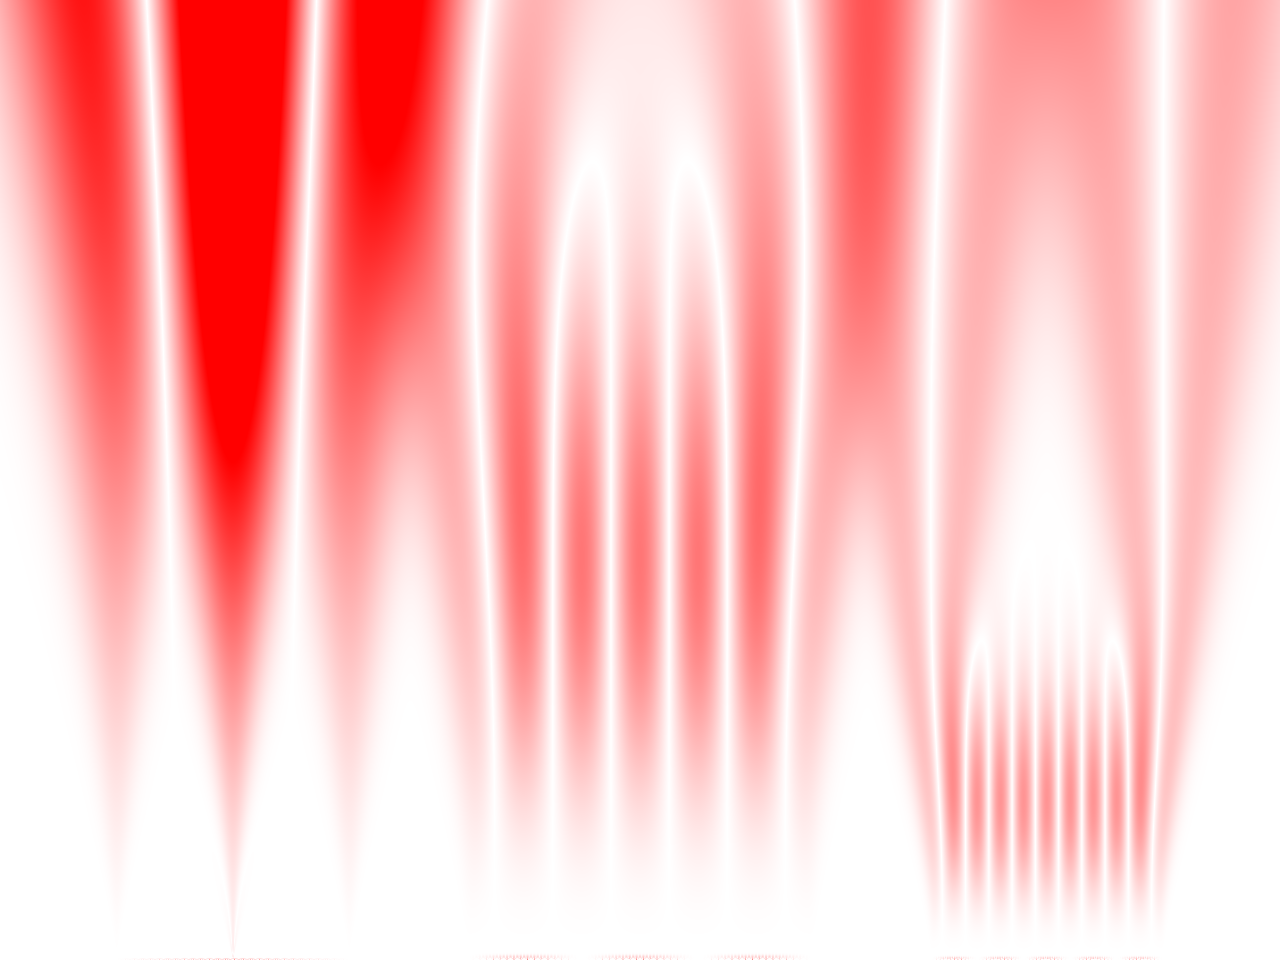
\includegraphics[width=9cm]{../../buch/chapters/4-cwt/images/notes.png}};

\draw[line width=1pt,color=blue]
	(-4.1,0)--(-3,0)--(-2,{2*2.883})--(-1,0)--(0,0)--
        plot[domain=0:3,samples=100] ({\x},{1.205*(1-cos(2*180*\x))})
        --(3,0)--(4,0)--
        plot[domain=4:6,samples=100] ({\x},{0.968*0.5*(1-cos(5*180*\x))})
        --(7.1,0);

\draw[->,line width=1pt] (-4.1,0)--(7.3,0) coordinate[label={$b$}];
\draw[->,line width=1pt] (0,-0.1)--(0,{0.75*11+0.3})
	coordinate[label={right:$a$}];

\draw[line width=1pt] (-0.1,{0.3333*0.75*11})--(0.1,{0.3333*0.75*11});
\draw[line width=1pt] (-0.1,{0.6666*0.75*11})--(0.1,{0.6666*0.75*11});
\draw[line width=1pt] (-0.1,{1.0000*0.75*11})--(0.1,{1.0000*0.75*11});

\node at (-0.1,{0.3333*0.75*11}) [left] {$0.2$};
\node at (-0.1,{0.6666*0.75*11}) [left] {$0.4$};
\node at (-0.1,{1.0000*0.75*11}) [left] {$0.6$};

\foreach \x in {-4,...,7}{
	\draw[line width=1pt] ({\x},-0.1)--({\x},0.1);
}

\end{tikzpicture}
\end{center}
\end{frame}
}

%
% 
%
\begin{frame}
\frametitle{Analyse eines Sweep mit Morlet-Wavelet}
\begin{tabular}{ll}
\ifthenelse{\boolean{presentation}}{
\begin{minipage}{8.5cm}
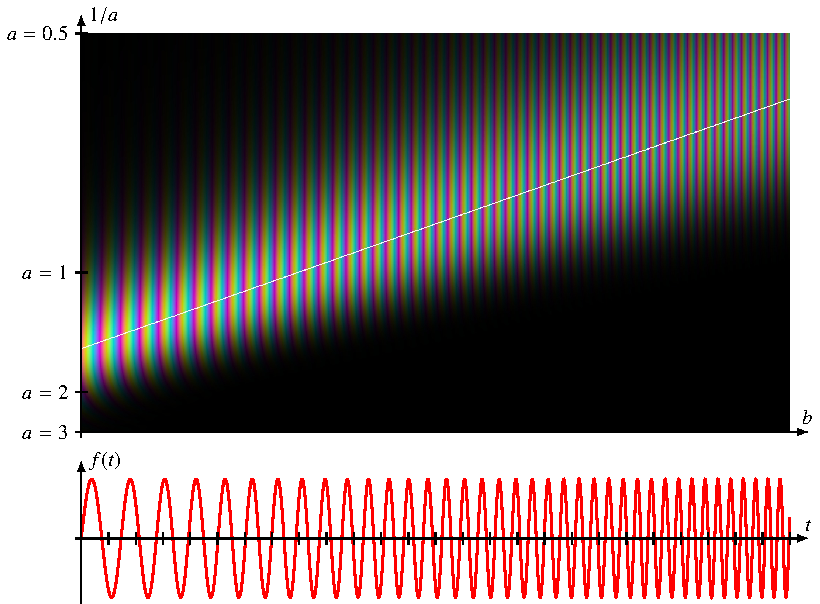
\includegraphics[width=\hsize]{../../buch/chapters/4-cwt/images/sweep.pdf}
\end{minipage}
}{
\begin{minipage}{9.5cm}
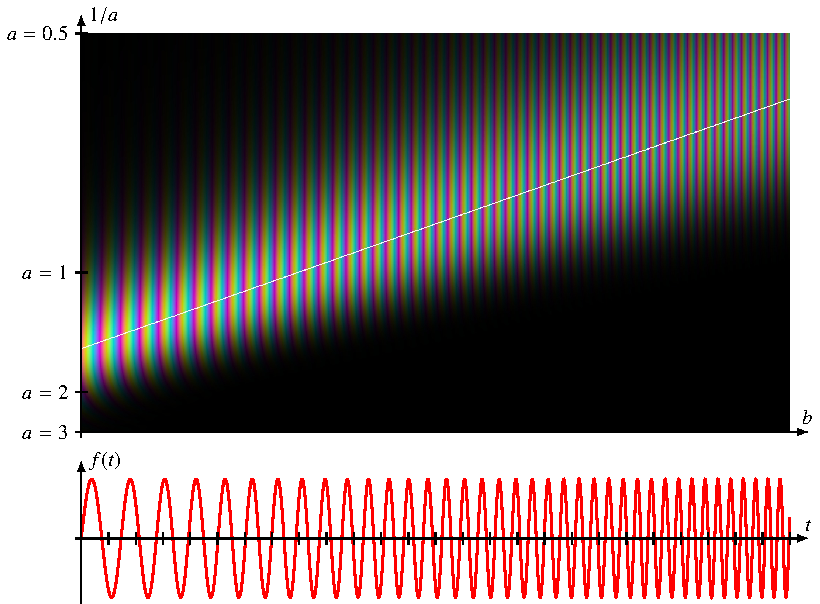
\includegraphics[width=\hsize]{../../buch/chapters/4-cwt/images/sweep.pdf}
\end{minipage}
}&%
\ifthenelse{\boolean{presentation}}{
\begin{minipage}{4.1cm}
Wavelet:
\[
\psi(t) = e^{-t^2/2} \cdot e^{5it}
\]
Signal:
\[
f(t)
=
\sin(t\cdot(4+0.2t))
\]
\end{minipage}
}{
\begin{minipage}{4.5cm}
Wavelet:
\[
\psi(t) = e^{-t^2/2} \cdot e^{5it}
\]
Signal:
\[
f(t)
=
\sin(t\cdot(4+0.2t))
\]
\end{minipage}
}
\end{tabular}
\end{frame}

%
% Eigenschaften der Transformation
%
\begin{frame}
\frametitle{Beobachtungen}
Eigenschaften von $\mathcal{W}$
\begin{itemize}
\item<2->
$\mathcal W$ ist linear\uncover<3->{:}
\begin{align*}
\uncover<4->{\mathcal{W}(f+g)} &\uncover<4->{= \mathcal{W}f + \mathcal{W}g}
\\
\uncover<5->{\mathcal{W}(\lambda f)} &\uncover<5->{= \lambda \mathcal{W}f}
\end{align*}
\item<6->
$\mathcal W$ ist injektiv \uncover<7->{ $\Rightarrow$ Umkehrformel?}
\item<8->
$\mathcal W$ ist nicht surjektiv
\end{itemize}
\end{frame}

%
% Definition zulässiger Wavelets
%
\begin{frame}
\frametitle{Wavelet}
\begin{definition}
Ein {\em Mutter-Wavelet} oder {\em Wavelet} ist eine Funktion
$\psi\colon\mathbb R\to\mathbb C$ mit
\[
\psi\in L^2(\mathbb R)
\qquad\text{und}\qquad
\|\psi\|=1,
\]
welche zudem die Zulässigkeitsbedingung erfüllt.
\end{definition}

\theoremstyle{definition}
\newtheorem{zulassig}{Zulässigkeitsbedingung}
\begin{zulassig}
$\psi\in L^2(\mathbb R)$ heisst zulässig, wenn
\[
C_{\psi}
=
\int_{\mathbb R^*} \frac{|\hat{\psi}(\omega)^2|}{|\omega|}\,d\omega
<
\infty
\]
\end{zulassig}
Die Zulässigkeitsbedingung wird benötigt für die Umkehrformel.
\end{frame}
